\section{SE-PIM Objectives and Challenges}
In this section, we first establish the design objectives of \thename. We then explain the generalized baseline PIM architecture, on which \thename's design proposals construct confidential computing capabilities. Against the threat model, which is also explained in this section, we explain the unique challenges that our design must mitigate. 


% describe the threat model in \cref{subsec:threat-model}. 
% We describe a generalization of PIM architectures, which we refer to as \baseline (\cref{subsec:pim-baseline}).

% Then, we illustrate the challenges in achieving our objectives, even the design additions to \baseline for confidential computation in~\cref{subsec:challenges}.


\subsection{Design Objectives of SE-PIM}
\label{subsec:objectives}
Our goal is to enable the memory to actively cooperate with a CPU-based enclave to perform confidential computation. Hence, our system functions as a secure memory extension for the host enclave and a secure accelerator for data-intensive computation. We identify the high-level objectives for \thename as follows. 

\hdr{\thename is a trusted memory extension.} \label{g2} 
One of the \thename's objectives is to function as a secure memory extension that supplements the limited memory capabilities of secure enclaves. The memory limitation of secure enclaves is a substantial problem that impedes the widespread adoption of confidential computing for large data. Many works proposed partitioning large data into batches that fit into the enclave memory space, but at the cost of performance~\cite{bigmatrix,occulemency}. On the other hand, turning memory into an active entity in secure data storage and processing can solve the problem of limited memory space in cloud enclaves. 



\hdr{\thename is a secure large data computation accelerator.} \label{g3} 
PIM-enabled memory devices are on the horizon~\cite{samsung-pim,amd-hbm,upmem,pim-architecture} and their advantages in accelerating data-intensive cloud workloads have been demonstrated~\cite{upmem-atc,upmem-benchmark,scalable-pim-acc,nda,pim-architecture}. Our objective is to take advantage of the processing capability of PIM by allowing the host enclaves to launch a protected PIM kernel on \thename-enabled memory banks. Furthermore, our hardware modifications must not introduce significant overhead to PIM computation.
 
We observe that PIM can inherently reduce the attack surface to many side-channel attacks that have been an existential threat to many processor enclaves~\cite{sgx-cache-attack,leaky-cauldron,sgx-page-table}. Performing computations where the data resides eliminates side-channels that occur while the data moves in a route on the memory bus or stored in shared storage, such as the processor caches~\cite{sgx-cache-attack}. We observe that such \emph{zero-copy} data transfer in PIM-assisted computations eliminates \emph{runtime} data movement between the CPU and PIM, thereby inherently minimizing the address side-channels on the memory bus~\cite{drama,membuster}. 

% However, as we illustrate in \cref{subsec:challenges}, there can be subtle side-channels incurred from the \emph{memory content change} that can leak sensitive information about the PIM kernel execution. 


% We carefully analyze the attack vectors when designing \thename as a secure memory extension. We explain in \cref{subsec:challenges} that simply encrypting the memory content is insufficient against the attack vectors that exploit the data \emph{access pattern} to leak information. We also show that memory integrity is not fully protected even with authenticated encryption such as AES-GCM.

% \hdr{Security objectives and scope.} 
% \thename provides a secure computation offloading model between a processor enclave and a \thename-enabled memory module. A secure connection with the processor enclave is established through remote attestation. We protect the integrity and confidentiality of the data used by \thename and the host enclave. We also guarantee the elimination of observable access patterns to the in-\thename data from both the CPU-side enclave and \thename units in each bank. We only trust the \thename units which include our hardware modifications, and CPU-based enclaves. Other software and hardware components in the system are distrusted. Side-channel attacks on the host CPU that take advantage of microarchitectural characteristics are out of the scope of our protection. The host enclave can offload sensitive operations to \thename units to reduce the attack surface. We also consider the electromagnetic side-channel and power side-channel of \thename out-of-scope~\cite{power-side-channel-accelerator}. The row hammer attacks are also not considered.

% \hdr{Attacker capabilities.}
% The primary objective of the adversaries is to extract sensitive information protected by secure enclaves through powerful attacks that they can launch with kernel privilege and physical access. As the privileged software manages the memory mapping, a malicious system software could map a region of physical memory into its own memory space or to a malicious process memory space. This also allows the attacker to passively or actively tap into every I/O communication with DMA buffers of MMIO from the host with the PIM device. 

% With physical and privileged software accesses to the system, an attacker can perform physical attacks on the MMIO interface of devices and the memory system. The attacker might corrupt the packet by tampering with the payload. They might also replay or delay a previously valid packet on the bus. The attacker could perform access pattern analysis to infer sensitive information from the memory accesses or MMIO packets \cite{access-pattern-disclosure,membuster}. We also consider \emph{DMA attacks} \cite{write-access-pattern}, where an attacker takes snapshots of the memory content at a high frequency to extract the changes in memory. \emph{Cold boot} attacks, where an attacker exploits the memory retention behavior of DRAM to extract the content of memory directly, are also considered~\cite{coldboot-attack}. 

\subsection{Baseline PIM}   
Prior to explaining the challenges in retrofitting a PIM architecture to have confidential computing capabilities, we first explain a generalized PIM architecture without support for confidential computing and its programming model, named \baseline. Using the \baseline architecture, we explain the challenges in \thename's imperative additions to \baseline for confidential computing.

\hdr{\baseline architecture.} Our baseline PIM model (\baseline) is a generalization of several works that introduces compute capabilities to memory~\cite{upmem-atc,tesseract}. We assume that in each memory bank of a memory module (e.g., 3D-stacked memory or DIMM memory stick), there is an integration of a programmable processing core (i.e., the \emph{PIM core}). The PIM cores can execute PIM kernels, program binaries compiled to run on a PIM core. As to the processing capacity of these processors, they often lack processor caches~\cite{upmem,smcsim,top-pim,neural-network-training}, and packaged with a low-latency on-chip memory, or \emph{PIM local memory}~\cite{smcsim,upmem,cho2020accelerating}. The local memory stores the PIM kernel and data a PIM core operates on. The PIM core accesses data inside a memory bank thorough \emph{direct memory access} (DMA). It requests the on-chip DMA engine to fetch batches of data into its local memory and process the data there. We do not assume architectural support for cache coherency between the PIM core and the host processor. A cache coherence scheme often requires PIM-aware changes to the host processor architectures~\cite{pei,conda}. Therefore, our current design does not involve concurrent computation on the same data between the PIM core and host processor.


\label{subsec:pim-baseline}
\begin{figure}[t]
    \centering
    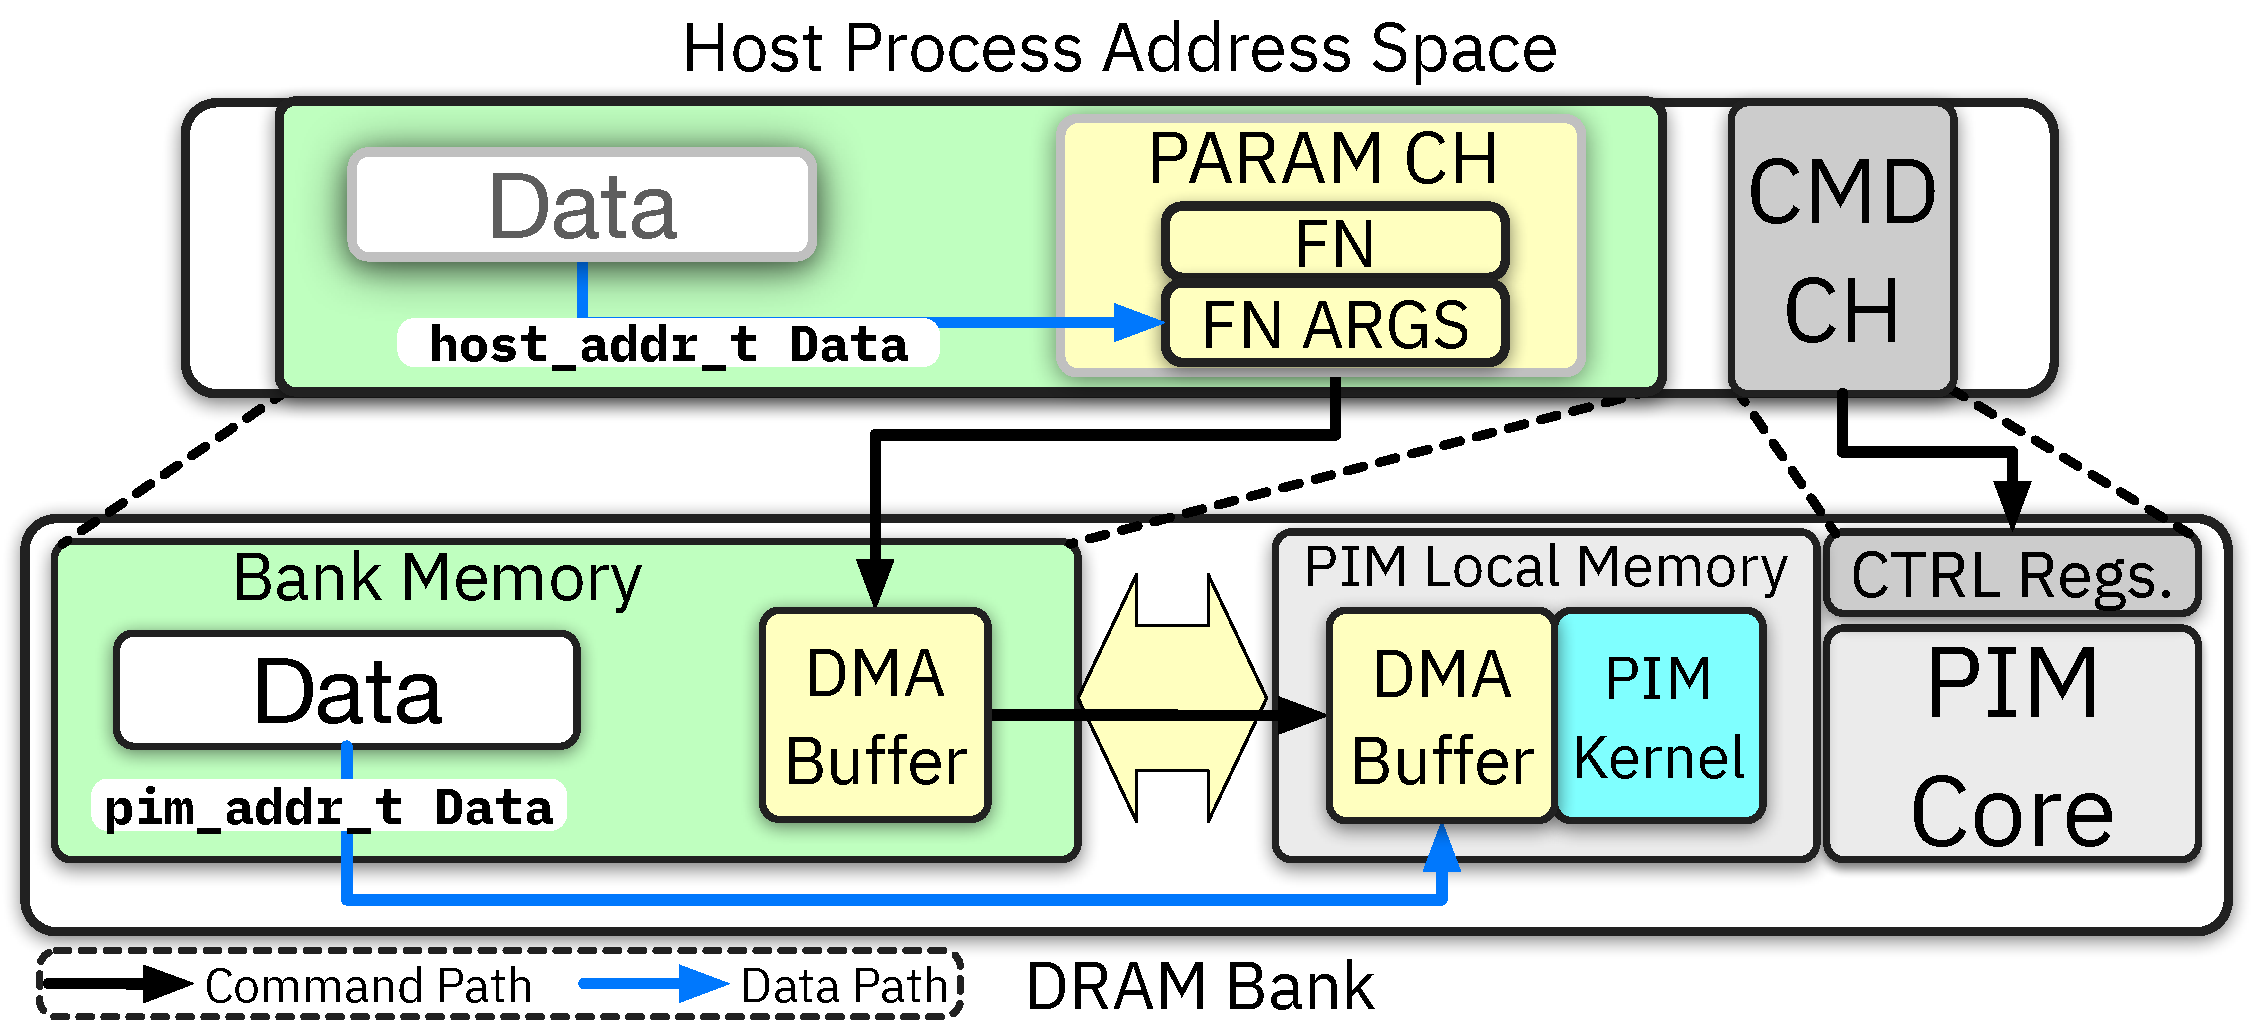
\includegraphics[width=.9\columnwidth]{figures/sepim/interfaces.pdf}
    \caption{The communication interfaces between the host and PIM using mappings of memory in host process address space.}
    \label{fig:interfaces}
\end{figure}

\hdr{Host-side access to memory.}
The memory bank of \baseline can be used as the normal memory space for the host program. We assume a direct mapping approach for data transfer between the host process and PIM-enabled memory banks; the physical address space of the memory bank is mapped by the driver into a contiguous address range in the host process (demonstrated in \autoref{fig:interfaces}). The CPU uses the mapped addresses to transfer data into the memory bank directly (the \emph{data channel}). We assume an uncached mapping for the PIM memory banks for data coherency between the host CPU and PIM such that the memory modifications in the host are immediately visible to PIM. \baseline must also support address translation on the PIM core, because the host and PIM uses different address spaces. To achieve this, the PIM core and the host process share a contiguous memory range with a direct mapping scheme, a common design seen in PIM designs~\cite{tesseract}. The PIM core can obtain the in-bank physical address from the host virtual address through a constant offset (\texttt{pim\_addr} $=$ \texttt{host\_addr} $-$ \texttt{C}), for all shared addresses. 

\hdr{Interfaces between host and PIM.}
A host program is typically employed to control the execution of the PIM cores. Similar to most I/O devices, the host process and \baseline communicate using two interfaces, MMIO registers, and DMA. For MMIO-based communications, the PIM system exposes registers to the host, which are used to send \emph{commands} to the PIM units to control their execution. We refer to this as the \emph{command channel} (CMD CH in \autoref{fig:interfaces}). DMA-based communication in \baseline copies data within the memory bank into PIM local memory using the fast PIM bus close to the memory. Hence, PIM-based DMA is different from the DMA communication of other devices that requires data to move across the slow peripheral buses. The host uses the DMA buffer to send \emph{parameters}, a data structure containing arguments for the PIM kernel (e.g., pointers to data inside memory) and commands. We refer to this channel for communication as the \emph{parameter channel} (PARAM CH in \autoref{fig:interfaces}). In order to utilize PIM, the host program loads the PIM kernel into PIM local memory (typically via MMIO~\cite{upmem-atc,smcsim}), writes the parameters that have the function name and its arguments into the parameter channel, and sends a command to the command channel to start executing the PIM kernel. The PIM core then fetches the parameters into its local memory and executes the requested function with the arguments.

\hdr{Zero-copy data exchange.} PIM computations typically utilize \emph{zero-copy} data exchanges. As demonstrated in \autoref{fig:interfaces}, the PIM kernel takes \emph{pointers} to data already located within memory as the arguments for execution. The PIM kernel uses the pointers as the source address to fetch data into the local memory for processing with efficient DMA transfers. With zero-copy, data exchanges on the slow memory bus are reduced, and efficiency is achieved in terms of bandwidth utilization and CPU cycles~\cite{pointer-chasing,smcsim,primer-on-pim}.


\subsection{Threat Model}
\label{subsec:threat-model}
%\hjc{check}
We protect the integrity and confidentiality of the data used by \thename and the host enclave. We also guarantee the elimination of observable access patterns to the in-\thename data on the memory bus. We only trust the \thename-enabled memory that contains our hardware modifications and CPU-based enclaves. Other software and hardware components in the system (e.g., the OS and other applications) are distrusted. Side-channel attacks on the host CPU that take advantage of microarchitectural characteristics are out of our protection scope. The host enclave can offload sensitive operations to \thename units to reduce the attack surface. We also consider the electromagnetic side-channel and power side-channel of \thename out-of-scope~\cite{power-side-channel-accelerator}. The row hammer attacks are also not considered.

%\hjc{Explain the trusted components }
Regarding the security of the PIM itself, we assume that the tightly integrated PIM-enabled memory bank, which includes the PIM core, PIM local memory, and our introduced modifications, are secure from physical attacks. The connections inside the PIM hardware are often connected with highly integrated connections (e.g., Silicon Vias (TSV)), so we assume that using hardware probes to snoop data contents from PIM is infeasible.




\subsection{Challenges}
\label{subsec:limitations}
\label{subsec:attack-vectors}
\label{subsec:challenges}
% In this section, we illustrate the challenges in achieving our objectives depicted in \cref{sec:goals}. 

%We elaborate the assumptions we make on the baseline PIM to enable confidential computation. Then,  (described in \autoref{fig:attack-vectors}).

PIM exhibits many inherent strengths as a side-channel resistant confidential computing accelerator for host enclaves. However, the required design changes for PIM architectures have not been explored to the best of our knowledge. Our contribution lies in identifying the unique challenges and proposing a set of design changes for mitigating them.

We start by introducing rudimentary features that are essential for confidential computation into the aforementioned \baseline. Namely, we assume that the attestation and secure channel establishment capabilities are now in place, similar to previously proposed secure hardware accelerator architectures~\cite{graviton,trustore,invisimem}. This means that both parties -- the host enclave and PIM -- communicate through encrypted channels to exchange commands and data. The encrypted data is stored in the memory banks and only to be decrypted inside PIM local memory when the PIM core proceeds to process the data.

However, we see that there still remains critical challenges in securing the workload computation performed in cooperation of the host enclave and PIM. We rigorously inspect all attack vectors that may allow the adversary to leak information about the \thename-assisted confidential computation. \autoref{fig:attack-vectors} summarizes the challenges that we identify. In the rest of this section, we explain the challenges in depth.

% We point out an inherent performance limitation in the baseline PIM in achieving end-to-end encryption with the host enclave and illustrate our point with an evaluation of real PIM hardware. In addition, we observe the attack vectors that must be mitigated for a PIM to function as secure storage and accelerator. The attack vectors are illustrated in \autoref{fig:attack-vectors}.

%\autoref{fig:attack-vectors} displays the security challenges in \baseline that we must address in the design. 



\begin{figure}[h]
    \centering
    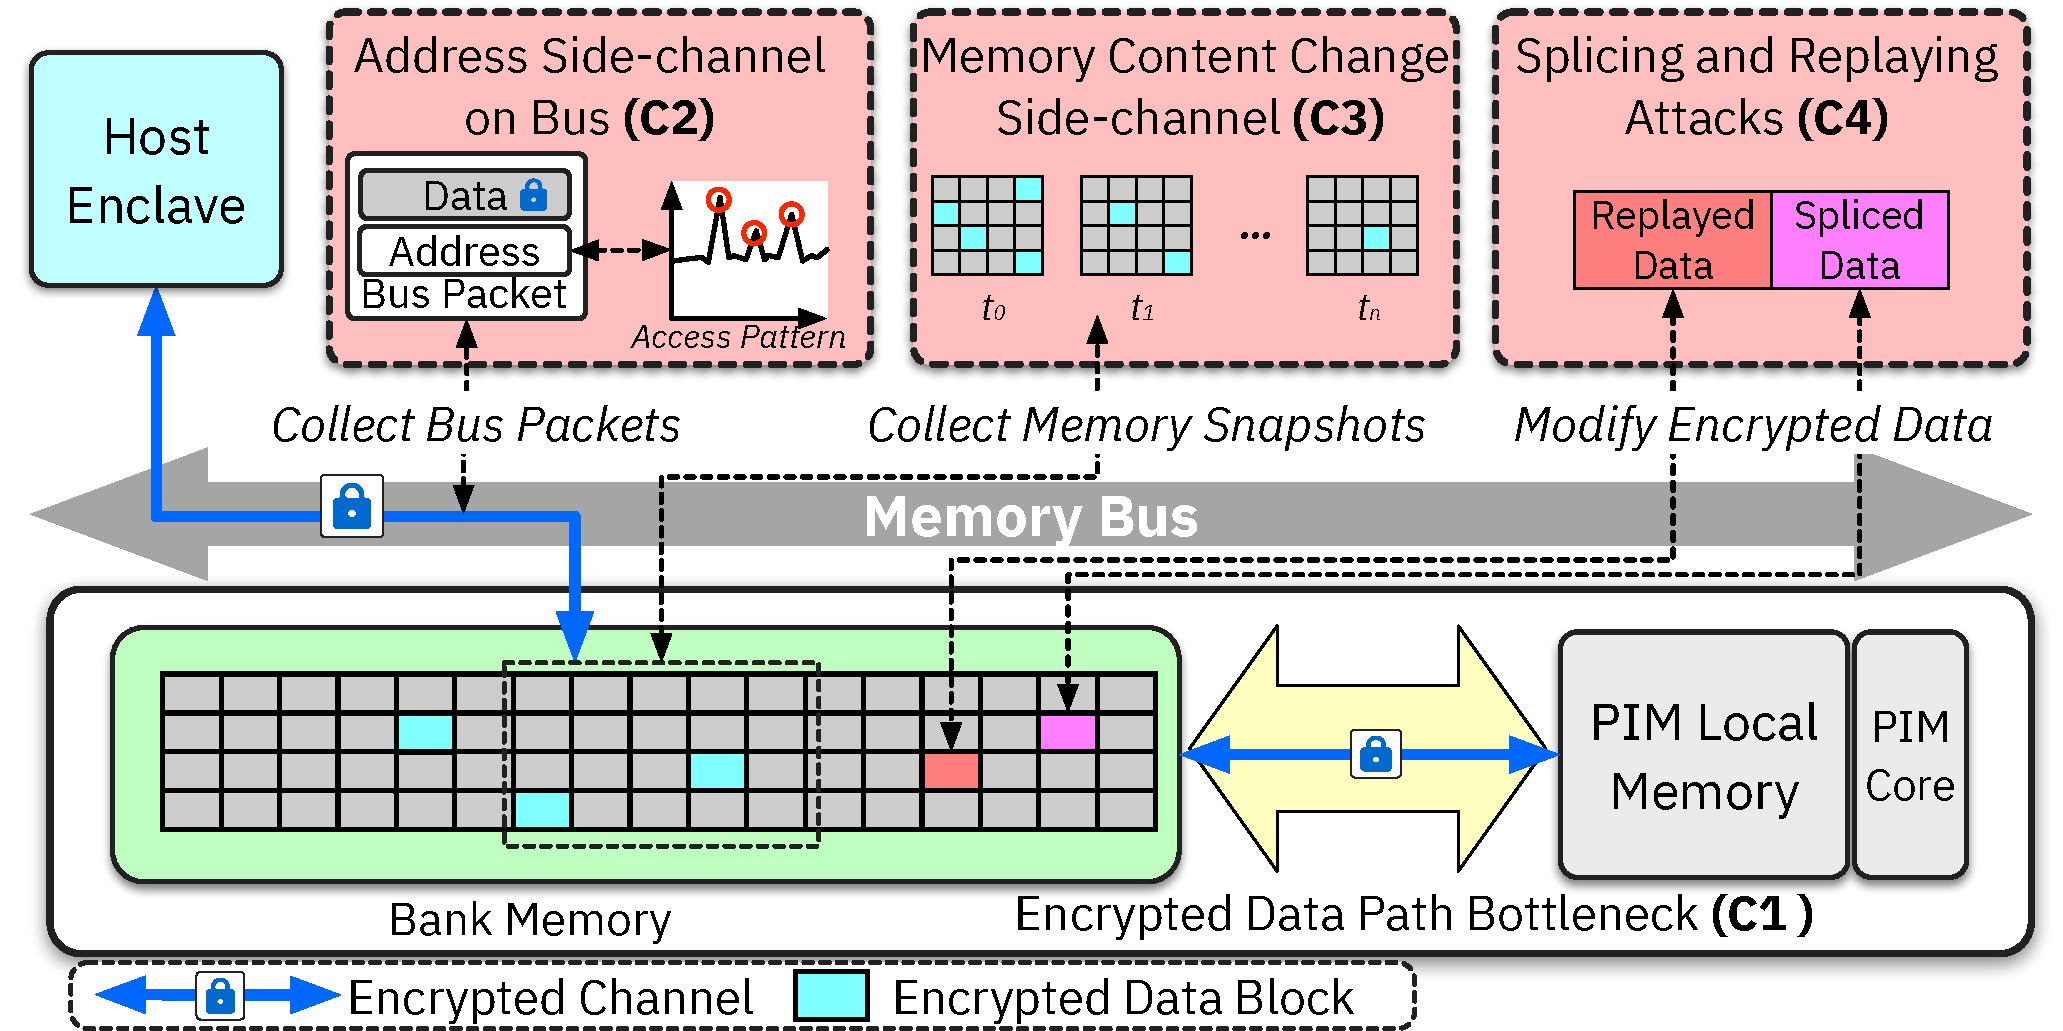
\includegraphics[width=0.8\textwidth]{figures/sepim/attack-vectors.pdf}
    \caption{Challenges faced by \baseline. Encrypted data movement between PIM local memory and the bank memory creates a performance bottleneck (C1). Memory accesses by the host enclave can leak the \emph{accessed address} on the bus (C2). An adversary can also monitor the memory content changes by quickly taking memory snapshots and comparing the differences (C3). Data inside memory is also vulnerable to splicing and replay attacks (C4).}
    \label{fig:attack-vectors}
\end{figure}
\begin{figure}[h]
    \centering
    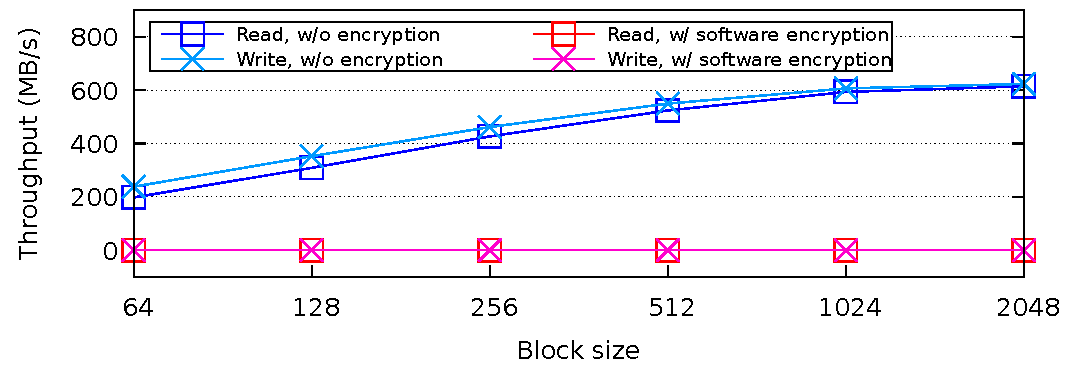
\includegraphics[width=.8\columnwidth]{figures/sepim/upmem-bandwidth.pdf}
    \caption{The memory throughput with and without software AES encryption on UPMEM PIM hardware.}
    \label{fig:upmem-aes}
\end{figure}



\newcommand{\challenge}[1]{\hyperref[c#1]{C#1}}

\newcommand{\attack}[1]{\hyperref[a#1]{A#1}}
\textbf{C1: Performance overhead of end-to-end encryption.}\label{c1}
It is essential that the command and data channels between the host and core are encapsulated with an end-to-end encrypted channel. However, we found that this is infeasible without hardware acceleration for encryption. To support our point, we evaluated the performance of working with encrypted data using software-based AES using \emph{mbedtls} on UPMEM’s real PIM hardware~\cite{upmem,upmem-atc}. The performance of encrypted DMA transfers is measured in both ways; the PIM core encrypts the data before transferring it from its local memory to the memory bank and decrypts the data as the data comes in the reverse direction. We measured the latency of each transfer from the initiation of encryption/decryption to the completion of the DMA transfer. 

As shown in \autoref{fig:upmem-aes}, software AES incurs immense performance overhead. The throughput plummeted from 600 MB/s to 0.5 MB/s, around 1200$\times$ lower throughput for both read and write. The results convinced us that hardware acceleration for symmetric key cryptography must be included for confidential computing in PIM design. Unlike convention accelerators (e.g., GPU), PIM designs have more constraints in terms of power and area constraints, which will always be limiting factors in PIM designs~\cite{amd-hbm,hmc,upmem-atc}. 
 
%PIM excels at memory-intensive HMC and HBM~\cite{hmc,amd-hbm}, and the power and area constraints 

\textbf{C2: Address side-channel on memory bus.} \label{c2}
We observe that when the host access PIM memory banks by writing to the memory mappings of \baseline, an attacker can capture the accessed physical addresses on the memory bus with a snooping device. The attack vector was shown exploitable even on SGX secure enclave, where the memory content is encrypted~\cite{membuster}. Although sequential data placement into the memory bank does not generate observable access patterns, host-side data accesses that are parts of the data processing computation can leak sensitive information about protected data. 
%or instance, the host application might retrieve or update a specific data block in the memory bank, which leaks differentiable patterns on the memory bus.% The elimination of such side-channel is necessary to satisfy the design objective \goal{2}. 

%\hjc{Accessing encrypted data is a challenge? from whose perspective?}
\textbf{C3: Side-channels from memory content changes.} \label{c3}
In \baseline, the memory bank mapping is managed by the kernel, which is untrusted in the threat model of secure enclaves. The untrusted kernel can directly access the memory content of \baseline through the memory mapping or map the bank memory into a malicious process's address space. On the other hand, an attacker-controller DMA device on the same system can also access the bank's content. Even though data inside the bank can be encrypted, an attacker can take snapshots of the memory and extract the changes in the memory content made by the PIM kernel. Due to the limited size of the PIM’s local memory, the PIM kernel must work with the encrypted data in batches, which is not necessarily sequential. A batch of data will be fetched from the memory bank to be decrypted and processed. Then, depending on the PIM kernel logic, the memory content might be updated with new values. Such operations may inadvertently create recognizable patterns in the eyes of the passive adversary. Research has shown that by only observing the memory change over time, attackers can recover sensitive information about the unencrypted data~\cite{write-access-pattern}. %This side-channel contradicts our design objective of enabling \thename as a secure accelerator (\goal{3}) by leaking information about the execution of the PIM kernel.


\textbf{C4: Providing protection against splicing and replaying attacks.} \label{c4}
With the same methods described in \challenge{3}, attackers can also modify the content of \baseline's memory banks.
Encrypting data with authenticated encryption algorithms (e.g., AES-GCM) protects encrypted data against direct tampering by attaching an authentication tag to the encrypted data. However, data inside memory is susceptible to \emph{splicing} and \emph{replaying} attacks when external entities modify the encrypted data. The splicing attack replaces data from one location with a valid encrypted data block from another location. The replaying attack reverts a chunk of encrypted data to a previously valid state. Both attacks trick the integrity checking of authenticated encryption algorithms into verifying that maliciously crafted data blocks have not been tampered with. Compromising data integrity might also affect the correct execution of the PIM kernel; PIM might use outdated data or data from an incorrect location for processing. Hence, the attacks jeopardize the objectives of \thename both as a secure memory extension and a secure accelerator. The mitigation of replaying and splicing attacks typically requires additional metadata storage (e.g., the latest timestamp of each data block) and additional verification procedures that would inadvertently introduce overheads to each memory access~\cite{bonsaimerkletree,common-counter}. 

